
\documentclass[10pt,a4paper]{article}
\usepackage[margin=1.55cm]{geometry}
\usepackage[T1]{fontenc}
\usepackage[utf8]{inputenc}
\usepackage[dutch]{babel}
\usepackage{amsmath,amssymb}
\usepackage{tikz}
\usepackage{xcolor}
\usepackage{newtxtext,newtxmath}
\usetikzlibrary{arrows.meta,calc,positioning,decorations.pathmorphing}

\setlength{\parindent}{0pt}
\setlength{\parskip}{0.45em}

\definecolor{noteGreen}{RGB}{39,145,75}
\definecolor{noteBlue}{RGB}{38,93,180}
\definecolor{noteRed}{RGB}{210,55,76}
\definecolor{notePurple}{RGB}{130,50,160}

\newcommand{\uncertain}[1]{\textit{\textcolor{gray}{#1}}}
\newcommand{\atomcore}{
  \fill[noteRed!75] (-0.18,0.05) circle (0.19);
  \fill[noteRed!75] ( 0.18,0.05) circle (0.19);
  \fill[yellow!80!orange] (0,-0.22) circle (0.17);
  \fill[yellow!80!orange] (0, 0.30) circle (0.17);
  \draw[black!65] (-0.18,0.05) circle (0.19);
  \draw[black!65] ( 0.18,0.05) circle (0.19);
  \draw[black!65] (0,-0.22) circle (0.17);
  \draw[black!65] (0, 0.30) circle (0.17);
}
\newcommand{\shells}[1]{
  \foreach \r in {0.62,0.92,1.28,1.70}{\draw[black!70,line width=.7pt] (0,0) circle (\r);}
  #1
}

\title{Notebook 2012 --- Pagina's 32--36}
\author{}
\date{}

\begin{document}
\maketitle
\uncertain{Transcriptie en TikZ-reconstructie van de handgeschreven scans. Formules en labels zijn zo letterlijk mogelijk behouden; enkele lastig leesbare woorden zijn expliciet als onzeker aangeduid.}

\clearpage
\section*{Pagina 32 --- Statisch en geëxciteerd atoom}

\begin{minipage}[t]{0.47\textwidth}
\subsection*{Statisch atoom}

\begin{center}
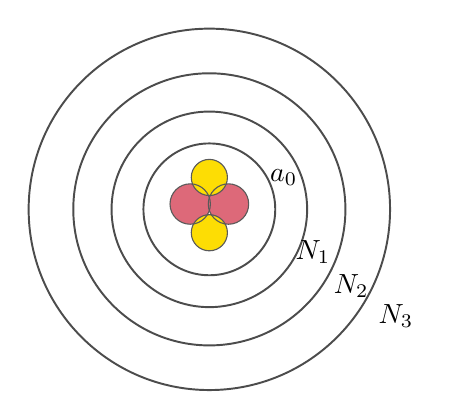
\begin{tikzpicture}[scale=1.35]
  \atomcore
  \shells{
    \node[right] at (0.48,0.30) {$a_0$};
    \node[right] at (0.72,-0.40) {$N_1$};
    \node[right] at (1.08,-0.72) {$N_2$};
    \node[right] at (1.50,-1.00) {$N_3$};
  }
\end{tikzpicture}
\end{center}

De schets toont een compacte kern met daaromheen opeenvolgende banen of schillen:
\[
a_0,\qquad N_1,\qquad N_2,\qquad N_3.
\]
\end{minipage}
\hfill
\begin{minipage}[t]{0.49\textwidth}
\subsection*{Excitatietoestand van het atoom}

\begin{center}
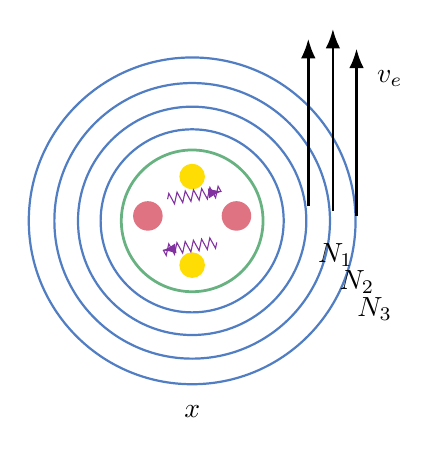
\begin{tikzpicture}[scale=1.25,>=Latex]
  \fill[noteRed!70] (-0.45,0.05) circle (.15);
  \fill[noteRed!70] ( 0.45,0.05) circle (.15);
  \fill[yellow!80!orange] (0,.45) circle (.13);
  \fill[yellow!80!orange] (0,-.45) circle (.13);
  \draw[noteGreen!70,line width=1.0pt] (0,0) circle (.72);
  \foreach \r in {0.93,1.16,1.40,1.66}{
      \draw[noteBlue!80,line width=.8pt] (0,0) circle (\r);
  }
  \draw[notePurple,decorate,decoration={zigzag,segment length=3pt,amplitude=2pt},->]
       (-.25,.22) -- (.30,.30);
  \draw[notePurple,decorate,decoration={zigzag,segment length=3pt,amplitude=2pt},->]
       (.25,-.22) -- (-.30,-.30);
  \draw[->,line width=.9pt] (1.18,.15) -- (1.18,1.85);
  \draw[->,line width=.9pt] (1.43,.10) -- (1.43,1.95);
  \draw[->,line width=.9pt] (1.67,.05) -- (1.67,1.75);
  \node[right] at (1.78,1.45) {$v_e$};
  \node[right] at (1.18,-.35) {$N_1$};
  \node[right] at (1.40,-.62) {$N_2$};
  \node[right] at (1.58,-.90) {$N_3$};
  \node[below] at (0,-1.78) {$x$};
\end{tikzpicture}
\end{center}

\uncertain{Handgeschreven tekst, waarschijnlijk:}

\begin{quote}
``Lichtsnelheid tijdens quantum-excitatie is een constante''
\end{quote}

\[
v_e = 1{,}0938456336 \cdot 10^6\ \mathrm{m\,s^{-1}}.
\]

\uncertain{Daaronder: ``$N$ is een meervoud van de ground-state-Bohr''.}
\end{minipage}

\clearpage
\section*{Pagina 33 --- Van $v_e$ naar $F_{\max}$}

\begin{minipage}[t]{0.47\textwidth}
\subsection*{Basisrelaties}

\begin{align*}
v_{\text{snelheid}}
  &= \omega_{\text{hoeksnelheid}}\,R_{\text{radius}},\\
\omega_{\text{hoeksnelheid}}
  &= \sqrt{\frac{k_{\text{springconstante}}}{m_{\text{massa}}}},\\
k_{\text{springconstante}}
  &= \frac{F_{\max}}{x}.
\end{align*}

\begin{center}
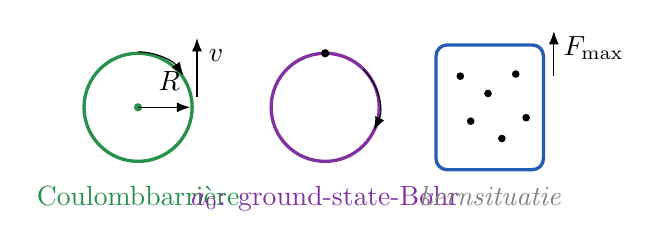
\begin{tikzpicture}[scale=.88,>=Latex]
  % situatie 1
  \draw[noteGreen,line width=1.2pt] (-2.7,0) circle (.78);
  \fill[noteGreen] (-2.7,0) circle (.06);
  \draw[->] (-2.7,0) -- (-1.95,0);
  \node[above] at (-2.25,.1) {$R$};
  \draw[->] (-1.85,.15) -- (-1.85,1.0);
  \node[right] at (-1.82,.75) {$v$};
  \draw[->] (-2.70,.80) arc[start angle=90,end angle=35,radius=.80];
  \node[noteGreen,below] at (-2.7,-1.0) {Coulombbarrière};

  % situatie 2
  \draw[notePurple,line width=1.2pt] (0,0) circle (.78);
  \fill[black] (0,.78) circle (.06);
  \draw[->] (.55,.55) arc[start angle=45,end angle=-25,radius=.78];
  \node[notePurple,below] at (0,-1.0) {$a_0$: ground-state-Bohr};

  % situatie 3
  \draw[noteBlue,line width=1.2pt,rounded corners] (1.6,-.9) rectangle (3.15,.9);
  \foreach \x/\y in {1.95/.45,2.35/.2,2.75/.48,2.1/-.2,2.55/-.45,2.9/-.15}
    {\fill[black] (\x,\y) circle (.055);}
  \draw[->] (3.3,.45) -- (3.3,1.10);
  \node[right] at (3.3,.85) {$F_{\max}$};
  \node[noteBlue,below] at (2.38,-1.0) {\uncertain{kernsituatie}};
\end{tikzpicture}
\end{center}

\begin{center}
\textcolor{noteRed}{``de 3 situaties''}
\end{center}
\end{minipage}
\hfill
\begin{minipage}[t]{0.49\textwidth}
\subsection*{Algebraïsche herschikking}

De notitie begint bij
\[
v=\sqrt{\frac{k}{m}}\,R.
\]

Met $k=F_{\max}/x$ en een radiusnummer $N$:
\begin{align*}
v
  &= \sqrt{\frac{F_{\max}}{xm}}\;R\,N,\\
v^2
  &= \frac{F_{\max}R_c^2N^2}{xm}.
\end{align*}

Daaruit volgen de opeenvolgende vormen uit de scan:
\begin{align*}
\frac{xmv^2}{N^2} &= F_{\max}R_c^2,\\
\frac{mv^2}{N^2} &= \frac{F_{\max}R_c^2}{x},\\
\frac{x}{N^2} &= \frac{F_{\max}R_c^2}{mv^2},\\
x &= N^2\frac{F_{\max}R_c^2}{mv^2}.
\end{align*}

\begin{center}
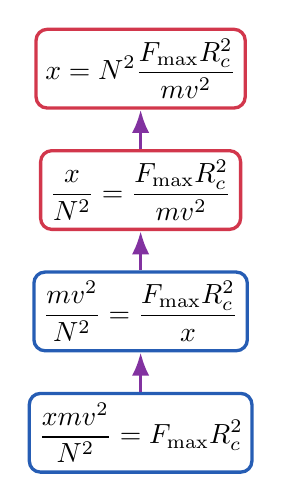
\begin{tikzpicture}[node distance=5mm,>=Latex]
\node[draw=noteBlue,very thick,rounded corners,align=center] (a)
{$\displaystyle \frac{xmv^2}{N^2}=F_{\max}R_c^2$};
\node[draw=noteBlue,very thick,rounded corners,above=of a] (b)
{$\displaystyle \frac{mv^2}{N^2}=\frac{F_{\max}R_c^2}{x}$};
\node[draw=noteRed,very thick,rounded corners,above=of b] (c)
{$\displaystyle \frac{x}{N^2}=\frac{F_{\max}R_c^2}{mv^2}$};
\node[draw=noteRed,very thick,rounded corners,above=of c] (d)
{$\displaystyle x=N^2\frac{F_{\max}R_c^2}{mv^2}$};
\draw[->,very thick,notePurple] (a)--(b);
\draw[->,very thick,notePurple] (b)--(c);
\draw[->,very thick,notePurple] (c)--(d);
\end{tikzpicture}
\end{center}

\uncertain{Bovenaan staat bovendien: ``als $v=v_e$, dan $x=a_0$''.}
\end{minipage}

\clearpage
\section*{Pagina 34 --- Veerconstante en $n$-bollen}

\begin{minipage}[t]{0.47\textwidth}
\subsection*{Springconstante}

\begin{center}
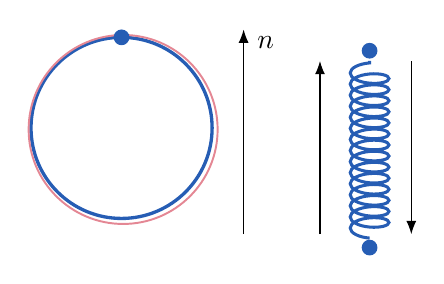
\begin{tikzpicture}[scale=1.0,>=Latex]
  \draw[noteBlue,line width=1.2pt] (-1.7,.3) circle (1.15);
  \draw[noteRed!60,line width=.7pt] (-1.68,.28) circle (1.20);
  \fill[noteBlue] (-1.7,1.45) circle (.10);
  \draw[->] (-.15,-1.05) -- (-.15,1.55);
  \node[right] at (-.10,1.38) {$n$};

  \draw[decorate,decoration={coil,aspect=.38,segment length=4pt,amplitude=7pt},
        noteBlue,line width=1.1pt] (1.45,-1.1) -- (1.45,1.15);
  \fill[noteBlue] (1.45,-1.22) circle (.10);
  \fill[noteBlue] (1.45,1.28) circle (.10);
  \draw[->] (.82,-1.05) -- (.82,1.15);
  \draw[<-] (1.98,-1.05) -- (1.98,1.15);
\end{tikzpicture}
\end{center}

\[
k=\frac{F_{\max}}{a_0}.
\]

\uncertain{Groene notitie: waarschijnlijk ``voor foton: de binding in de kern''.}
\end{minipage}
\hfill
\begin{minipage}[t]{0.49\textwidth}
\subsection*{$n$-bol --- Euclidische geometrie}

\begin{center}
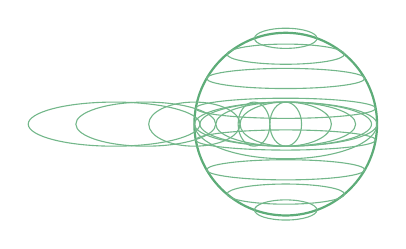
\begin{tikzpicture}[scale=.80]
  \draw[noteGreen!75,line width=.8pt] (0,0) circle (1.45);
  \foreach \a in {0,20,...,160}
    {\draw[noteGreen!65] ({1.45*cos(\a)},0)
      arc[start angle=0,end angle=360,x radius={abs(1.45*cos(\a))},y radius=.35];}
  \foreach \a in {-70,-50,...,70}
    {\draw[noteGreen!65]
      (0,{1.45*sin(\a)}) ellipse ({1.45*cos(\a)} and .16);}
  \draw[noteGreen!65] (-1.45,0) arc[start angle=180,end angle=360,x radius=1.45,y radius=.55];
\end{tikzpicture}
\end{center}

De voorbeelden zijn, op basis van de tekeningen:
\begin{align*}
0\text{-bol} &:\ \text{punt},\\
1\text{-bol} &:\ \text{lijnstuk met interieur},\\
2\text{-bol} &:\ \text{schijf met interieur},\\
3\text{-bol} &:\ \text{bollichaam met interieur}.
\end{align*}

\begin{center}
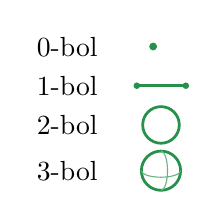
\begin{tikzpicture}[scale=.83]
  \node[left] at (-.2,1.15) {$0$-bol};
  \fill[noteGreen] (.5,1.15) circle (.06);

  \node[left] at (-.2,.55) {$1$-bol};
  \draw[noteGreen,line width=1pt] (.25,.55)--(1.0,.55);
  \fill[noteGreen] (.25,.55) circle (.05);
  \fill[noteGreen] (1.0,.55) circle (.05);

  \node[left] at (-.2,-.05) {$2$-bol};
  \draw[noteGreen,line width=1pt] (.62,-.05) circle (.28);

  \node[left] at (-.2,-.75) {$3$-bol};
  \draw[noteGreen,line width=1pt] (.62,-.75) circle (.30);
  \draw[noteGreen!70] (.32,-.75) arc[start angle=180,end angle=360,x radius=.30,y radius=.10];
  \draw[noteGreen!70] (.62,-1.05) arc[start angle=-90,end angle=90,x radius=.10,y radius=.30];
\end{tikzpicture}
\end{center}

\uncertain{Onderaan staat vermoedelijk $2n+1=\pm 7$ met het label ``torus vortex''.}
\end{minipage}

\clearpage
\section*{Pagina 35 --- Torus}

\begin{minipage}[t]{0.34\textwidth}
\subsection*{Dimensieschets}

\begin{align*}
0&\text{-torus},\\
1&\text{-torus},\\
2&\text{-torus},\\
3&\text{-torus}.
\end{align*}

\begin{center}
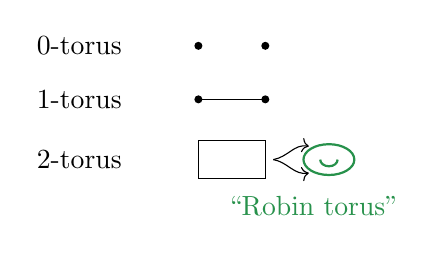
\begin{tikzpicture}[scale=.85]
  \node[left] at (0,1.65) {$0$-torus};
  \fill (1,1.65) circle (.06);
  \fill (2,1.65) circle (.06);

  \node[left] at (0,.85) {$1$-torus};
  \draw (1,.85)--(2,.85);
  \fill (1,.85) circle (.06);
  \fill (2,.85) circle (.06);

  \node[left] at (0,-.05) {$2$-torus};
  \draw (1,-.33) rectangle (2,.23);
  \draw[->] (2.12,-.05) to[out=10,in=170] (2.65,.15);
  \draw[->] (2.12,-.05) to[out=-10,in=190] (2.65,-.25);
  \draw[noteGreen,thick] (2.95,-.05) ellipse (.38 and .23);
  \draw[noteGreen,thick] (2.82,-.05) arc[start angle=180,end angle=360,x radius=.13,y radius=.10];
  \node[noteGreen,below] at (2.72,-.45) {``Robin torus''};
\end{tikzpicture}
\end{center}

\uncertain{De naam bij de kleine torusschets is niet volledig scherp; ``Robin torus'' is de waarschijnlijkste lezing.}
\end{minipage}
\hfill
\begin{minipage}[t]{0.62\textwidth}
\subsection*{Wireframe-reconstructie}

\begin{center}
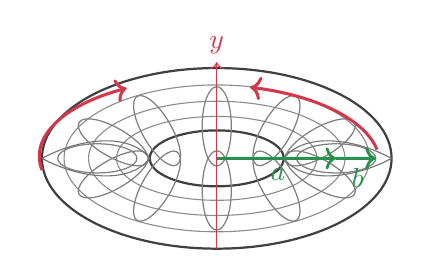
\begin{tikzpicture}[scale=.74]
  % Hoofdringen en silhouet
  \draw[black!75,line width=.8pt] (0,0) ellipse (3.0 and 1.55);
  \draw[black!75,line width=.8pt] (0,0) ellipse (1.15 and .48);
  \draw[black!45] (0,0) ellipse (2.62 and 1.26);
  \draw[black!45] (0,0) ellipse (2.20 and .98);
  \draw[black!45] (0,0) ellipse (1.72 and .72);

  % Dwarsdoorsneden rond de torus
  \foreach \a in {0,30,...,330}{
    \pgfmathsetmacro{\cx}{2.05*cos(\a)}
    \pgfmathsetmacro{\cy}{.55*sin(\a)}
    \draw[black!50,line width=.45pt,rotate around={\a:(\cx,\cy)}]
      (\cx,\cy) ellipse (.68 and .25);
  }

  % Extra meridianlijnen
  \draw[black!55] (-3,0) .. controls (-2.35,.35) and (-1.50,.45) .. (-1.15,0)
                  .. controls (-1.50,-.45) and (-2.35,-.35) .. (-3,0);
  \draw[black!55] (3,0) .. controls (2.35,.35) and (1.50,.45) .. (1.15,0)
                  .. controls (1.50,-.45) and (2.35,-.35) .. (3,0);

  \draw[->,noteRed,line width=1.1pt] (-3.0,-.2)
    arc[start angle=190,end angle=120,x radius=3.0,y radius=1.35];
  \draw[->,noteRed,line width=1.1pt] (2.75,.15)
    arc[start angle=10,end angle=75,x radius=3.0,y radius=1.35];
  \draw[->,noteGreen,line width=1pt] (0,0)--(2.05,0);
  \node[below,noteGreen] at (1.05,0) {$a$};
  \draw[->,noteGreen,line width=1pt] (2.05,0)--(2.73,0);
  \node[below,noteGreen] at (2.42,0) {$b$};
  \draw[->,noteRed] (0,-1.55)--(0,1.65);
  \node[above,noteRed] at (0,1.62) {$y$};
\end{tikzpicture}
\end{center}

De cirkel die de buisdoorsnede beschrijft is genoteerd als
\[
(x-a)^2+y^2=b^2.
\]

Daarbij verschijnen de buiten- en binnenstraal
\[
a+\sqrt{b^2-y^2},
\qquad
a-\sqrt{b^2-y^2}.
\]

Voor een torus met hoofdstraal $a$ en buisstraal $b$:
\begin{align*}
V &= 2\pi^2 a b^2,\\
A &= 4\pi^2 a b.
\end{align*}

\uncertain{In de scan staat bij het oppervlak $4\pi^2 R\cdot R$; de genormaliseerde torusformule hierboven gebruikt twee afzonderlijke stralen.}
\end{minipage}

\clearpage
\section*{Pagina 36 --- Inverse tangens en afgeleide}

\begin{minipage}[t]{0.35\textwidth}
\subsection*{Inverse functie}

De linkerhelft bevat:
\[
y=\tan^{-1}(x)
\quad\Longrightarrow\quad
\tan(y)=x.
\]
\end{minipage}
\hfill
\begin{minipage}[t]{0.61\textwidth}
\subsection*{Secanthelling}

\begin{center}
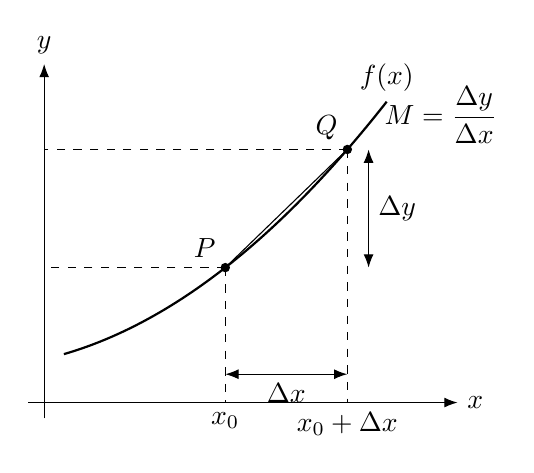
\begin{tikzpicture}[scale=1.0,>=Latex]
  \draw[->] (-.2,0)--(5.25,0) node[right] {$x$};
  \draw[->] (0,-.2)--(0,4.3) node[above] {$y$};

  \draw[thick,domain=.25:4.35,samples=100]
    plot (\x,{.55+.23*\x+.12*\x*\x}) node[above] {$f(x)$};

  \coordinate (P) at (2.3,{.55+.23*2.3+.12*2.3*2.3});
  \coordinate (Q) at (3.85,{.55+.23*3.85+.12*3.85*3.85});
  \fill (P) circle (.06) node[above left] {$P$};
  \fill (Q) circle (.06) node[above left] {$Q$};
  \draw[thin] (P)--(Q);

  \draw[dashed] (P)--(2.3,0) node[below] {$x_0$};
  \draw[dashed] (Q)--(3.85,0) node[below] {$x_0+\Delta x$};
  \draw[dashed] (P)--(0,{.55+.23*2.3+.12*2.3*2.3});
  \draw[dashed] (Q)--(0,{.55+.23*3.85+.12*3.85*3.85});

  \draw[<->] (2.3,.36)--(3.85,.36) node[midway,below] {$\Delta x$};
  \draw[<->] (4.12,{.55+.23*2.3+.12*2.3*2.3})
             --(4.12,{.55+.23*3.85+.12*3.85*3.85})
             node[midway,right] {$\Delta y$};
  \node[right] at (4.2,3.65) {$M=\dfrac{\Delta y}{\Delta x}$};
\end{tikzpicture}
\end{center}

De gemiddelde helling tussen $P$ en $Q$:
\[
M=\frac{\Delta y}{\Delta x}
 =\frac{f(x_0+\Delta x)-f(x_0)}{\Delta x}.
\]

In de limiet $\Delta x\to0$:
\[
\frac{dy}{dx}=f'(x).
\]
\end{minipage}

\end{document}
